\chapter{ARM V: Mathematicians' Adventures in Wonderland}

\hspace{\fill}\textbf{Isky Mathews}

\begin{multicols}{2}

Geometry problems are a staple of modern day maths tests, qualifications and olympiads---indeed, Euclid is considered perhaps the first modern mathematician, and his \textit{Elements}, used as a textbook for hundreds of years, predominantly focusses on geometric constructions on the plane. In fact, for many mathematicians in the 19th century, geometry in many dimensions was almost considered "solved", in that there were methods which could eventually given enough time understand all but a few objects. In some sense, geometry was the mathematical realisation of the real world for them and thus was a tool for physicists to describe and predict various aspects of it---they could never have predicted that there wasn't just \textbf{one geometry} and that many of these other geometries would have remarkable properties completely unlike that of Euclidean space. This article will mention the profound discovery of non-Euclidean geometries and focus on one particularly, known as \textit{hyperbolic geometry}, with some showcasing of even wilder beasts such as the quintic 3-folds of the complex projective space near the end...

\end{multicols}

\section{Journeys to the Hyperbolic}

\begin{multicols}{2}

Numerous people discovered hyperbolic geometry at around the same time, though interestingly in quite different contexts. One of the main trends of the era was to look into building a proper and rigorous foundation for contemporary mathematics, for it had been discovered that without exact definitions, clear axioms, and systematic work of this sort, one would soon find that mathematical questions could be asked that had no answer, simply because the concepts were too vague and so were not well-defined in all circumstances. The Hungarian mathematics student J\'{a}nos Bolyai was also interested in just this, looking particularly at Euclid's foundations of geometry. As many scholars of the time would tell you, Euclid put forth 5 main axioms:

\begin{itemize}
\item Given any two points, a straight line can be drawn connecting them.
\item A straight line can be continuously extended in either direction unboundedly.
\item All right angles are equivalent to each other.
\item Given a centre and a distance, a circle with that centre and with a radius of the given distance can be constructed.
\item Given a line \(A\) and a point \(B\) not on the line, there is exactly one new line \(C\) that can be drawn through the point so that \(C\) does not ever intersect \(A\).
\end{itemize}

If any of the above seems quite obvious to you, then that's good news! An \textit{axiom} is supposed to be a principle or truth that is considered so obvious that it does not require any proof; as such, mathematical theories or objects are typically begun with a list of such axioms making clear what is the topic of discussion. Euclid then went on in his book to describe various different geometric situations on the plane and prove various fundamental theorems used in geometry today, such as the fact that the interior angles of a triangle sum to 180\(^\circ\). However, what became clear to many reading this prized document was that in some sense, the fifth axiom or \textit{parallel postulate}, as it has come to be known, was significantly detached from the first four. This is because Euclid's first 25 or so theorems never used the fifth axiom whereas the others were used extensively---many wondered if it was actually possible to prove the fifth from the first four. When Bolyai read about this, he realised its importance and decided instead to attempt to prove that fifth axiom \textit{had} to be how it was because if it was any different, one would get an inconsistent (and thus, invalid) geometry; in other words, he tried a proof by contradiction. Amongst other things, he used this replacement of the parallel postulate, which appears at first glance to be faintly ridiculous:

\begin{itemize}
\item Given a line \(A\) and a point \(B\) not on the line, there are two lines \(C_1\) and \(C_2\) that can be drawn through the point so that neither ever intersect with \(A\).
\end{itemize}

So, Bolyai decided to start investigation this "non-geometry" and noticed amongst other things that triangles in this odd world can only have a sum of internal angles less than or equal to 180\(^\circ\). After this, he showed that in a quadrilateral with two equal-length sides \(A\) and \(B\) perpendicular to another side \(C\), the other two angles would be acute. As he went on proving theorem after theorem, it eventually occurred to Bolyai that in fact there was not a contradiction to be found---he and others after him succeeded in proving, astoundingly, that this new "hyperbolic" geometry was consistent if and only if Euclidean geometry was consistent (a belief commonly held by contemporary mathematicians).

Some of his other founding work included the description of the trigonometric functions for right-angled hyperbolic triangles (\(sinh(x), cosh(x)\) and \(tanh(x)\)) and proved some elementary identities concerning these. Furthermore, he showed that the "opposite" of his replacement of the parallel postulate, namely

\begin{itemize}
\item Given a line \(A\) and a point \(B\) not on the line, there are no lines that can be drawn through the point so that they never intersect with \(A\).
\end{itemize}

also defines a consistent geometry, called "elliptic geometry". On the elliptic plane, triangles always have \textbf{more} than 180\(^\circ\) as their sum of internal angles and tilings can be made such that a finite number of tiles cover the entire plane. It turns out that the elliptic plane is easily describable as the geometry on the surface of a sphere, where we represent a "point" as two opposite points (known as \textit{antipodal} points) on it and a line as a great circle of the sphere\footnote{A great circle on a sphere is one of the circles that one could draw on its surface such that the radius of the circle is equal to the radius of the sphere.}---so one of the tilings I mentioned can be seen as in \textbf{Fig. 3.1}, which is, by the way, analagous to the icosahedron.

Contemporaries of Bolyai, such as Lobachevsky and even Gauss himself, similarly independently discovered hyperbolic planes and geometry but through a different series of thoughts. It had occurred to them that on different surfaces from the flat plane one could also have a different geometry but classifying it was not as simple as it might appear. For example, a cylinder appears different from the plane; however, its surface has no distinct geometric properties; this can be seen by the fact that any figure or diagram on a Euclidean plane can be put on a cylinder, preserving angles and lengths. by picking up the plane and wrapping it around the cylinder like wallpaper (for example, toilet paper being on a roll). However, it is \textit{not} true that one can easily wrap a piece of paper around a sphere---one always finds wrinkles when doing so. Why is this? Gauss formulated the concept of Gaussian curvature to understand this and to aid his cartography of the Austrian Alps.

\end{multicols}

\begin{figure}[h]
\centering
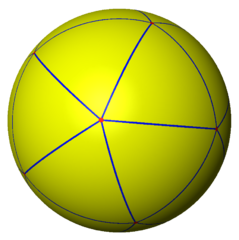
\includegraphics[scale=1]{Fig11}
\caption{A tiling of the elliptic plane.} 
\end{figure}

\begin{figure}[h]
\centering
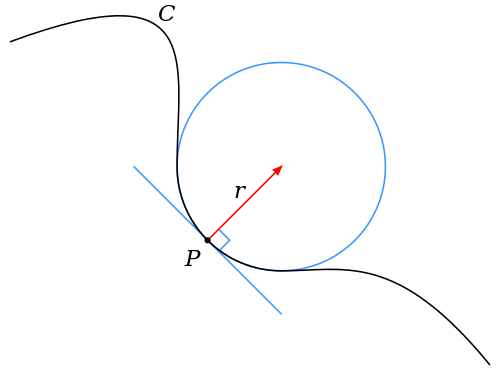
\includegraphics[width=0.5\textwidth]{Fig21}
\caption{A diagram of curvature at a point \(P\) with its "approximation circle" of radius \(r\).} 
\end{figure}

\begin{multicols}{2}

The curvature of a plane curve\footnote{ A plane curve can for our purposes be considered any line, wiggly or straight, drawn continuously on a surface.} at a specific point \(A\) can be considered intuitively as a measure of how effectively a tangent at \(A\) can be used to approximate the location of points just around \(A\) or how fast the tangent diverges from the actual curve as one moves away from \(A\). More rigourously, given any curve and a point \(A\) somewhere along it, there is a circle with a centre \(O\) on the line perpendicular to the tangent at \(A\) (called the \textit{normal}) with \(|OA| = r\) for some \(r\) (\(r\) is the radius). This is the best circle which approximates the curve for points close to \(A\)---an illustration of this concept can be seen in \textbf{Fig. 3.2}. We define \(\kappa\) to be the curvature, where \(\kappa = \frac{1}{r}\).

Using this, we can define Gaussian curvature, which is a way of measuring the intrinsic curvature of surfaces. Given a point \(A\) on a surface, consider the normal at \(A\) (here this is the perpendicular line to the \textit{tangent plane} at \(A\)) and then, further, consider all the planes that contain that normal. Each of the planes will intersect with a 1-dimensional cross-section of our surface, and so for each intersecting plane \(P_n\), we calculate the curvature of the corresponding 1-dimensional plane curve at \(A\), denoted \(\kappa_n\). Now, the \textit{Gaussian curvature} of \(A\) is defined to be the product of the maximum and minimum such \(\kappa_n\) (known as the \textit{principal curvatures} at the point \(A\)). So, let's stop to consider what the Gaussian curvature of various well-known surfaces looks like: 
\begin{itemize}
\item with a point on a plane, the curvature of a point on any plane-cross-section is 0, since the best circle which approximates a straight line has an infinitely large radius\footnote{In other words, \( \lim_{R \to \infty} \frac{1}{R} = 0\)}, so \(\kappa_{max}, \kappa_{min} = 0\), so the Gaussian curvature is 0; 
\item with a point on a cylinder, the curvature of the long straight axis is \(\kappa_{min}\) which is 0 for the same reason as on the plane and so regardless of \(\kappa_{max}\), its G. curvature is 0; 
\item with a point on a sphere, every plane-cross-section will be a circle of radius \(R\), meaning that \(\kappa_{min}, \kappa_{max} = \frac{1}{R}\) and so the G. curvature is \(\frac{1}{R^2}\) at every point.
\end{itemize}

\end{multicols}
 
\begin{figure}[h]
\centering
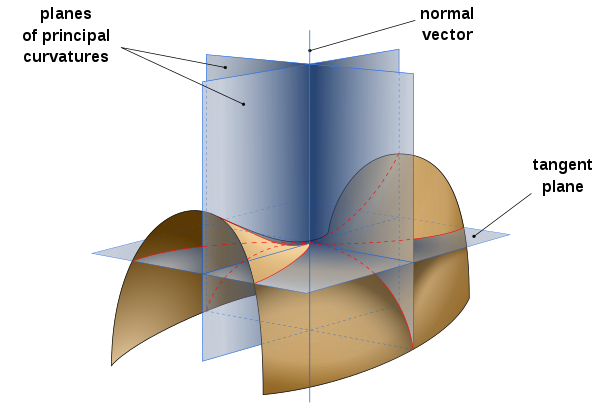
\includegraphics[width=0.5\textwidth]{Fig31}
\caption{A "saddle-surface".} 
\end{figure}

\begin{figure}[h]
\centering
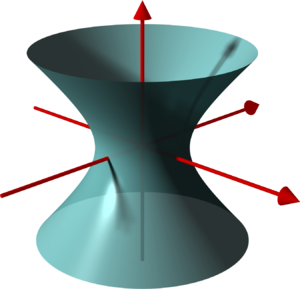
\includegraphics[scale=0.5]{Fig41}
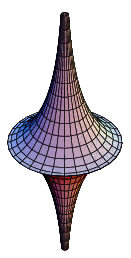
\includegraphics[scale=0.5]{Fig42}
\caption{A hyperboloid and a pseudosphere.} 
\end{figure}

\begin{multicols}{2}

What would a point of negative curvature on a surface look like? Consider \textbf{Fig. 3.3}, displaying a so-called "saddle-surface". At the centre of the saddle, the diagram displays the planes which intersect the surface at its principal curvatures---one of the cross-sections curves upwards in the direction of the normal and the other, 90\(^\circ\) to the first, curves downwards against the direction of the normal. The former would have some positive \(\kappa_{max}\) but since the other curves downwards from the normal, Gauss said it would be natural to assign the downwards curve a negative \(\kappa_{min}\) and so the Gaussian curvature (their product) would also be negative. The interesting question that Gauss asked after considering this was: what would a surface with constant negative curvature look like? After giving the problem some thought, one might come up with the surfaces shown in \textbf{Fig. 3.4}; one is a \textit{hyperboloid} (the surface of revolution of a hyperbola) and the other is called a \textit{pseudosphere}, discovered by Bolyai. Both have negative curvature at almost all of their points but neither have constant negative curvature.

In trying to understand the problem better, one can examine the geometric properties of such a surface, and what one discovers is that triangles have less than or equal to 180\(^\circ\) as their summed internal angles etc.---this is just a different description of the hyperbolic plane! Although Gauss never did gain much better insight into the nature of such a surface, he did prove the important \textit{Theorema Egregium} which says that by performing cutting, rotating, translating or bending operations on a surface, one sustains the same Gaussian curvature at every point; thus, Gaussian curvature is a defining "unalterable" property of a surface, showing clearly why one can't wrap a piece of paper around a sphere as easily as around a cylinder---the piece of paper has constant zero curvature, and the sphere has \(\frac{1}{R^2}\), and so to cover the sphere with paper, one would have to be able to stretch or otherwise fundamentally alter its nature. It also shows why rolling up a piece of paper into a cylinder makes it so much more rigid than when it was just flat: when you've rolled it up, you have created a positive curvature in one direction and so for the paper to retain its constant zero Gaussian curvature, it has to stay straight in the other direction...

The final piece of the puzzle came from the work of the prolific David Hilbert with \textit{Hilbert's Theorem}\footnote{It should be noted that this name, just like \textit{Euler's Theorem} in modular arithmetic, is completely ridiculous since the individual it's named after proved many hundreds of theorems and is commonly considered to be amongst the most important of mathematicians of the 19th and 20th centuries.}, which essentially proved that given an \(n\)-dimensional hyperbolic geometric space (as in, an \(n\)-space of constant negative curvature) there is no distance and angle-preserving way of putting it into an \(n\)-dimensional Euclidean space, certifying that this is a consistent and fundamentally distinct geometry.

\end{multicols}

\section{Schl\"{a}fli notation and tilings}

\begin{multicols}{2}

For those who read the first article in this series, you would have seen an introduction to some of the many combinatorial and geometric problems and properties of tilings of the Euclidean plane. It was suggested then that hyperbolic geometry sported a much greater collection of such tilings and now we shall see that such comments are quite justified and that, in some sense, most tilings are in fact hyperbolic. 

The \textit{Schl\"{a}fli symbol} \(\{x_2, x_1\}\) is a notation used to denote a tiling where there are \(x_1\) \(x_2\)-gons around a point. So, for example, the Schl\"{a}fli symbol \(\{4,4\}\) describes the classic square-lattice tiling on the Euclidean plane and \(\{3,5\}\) describes the tiling in \textbf{Fig. 3.1}. You might notice that this notation severely limits the number of tilings one can describe, since one can only notate those which use only 1 shape, and in which each vertex has the same number of polygons around it (these are known as the \textit{regular tilings}), but it is still useful. What symbols \(\{p,q\}\) are Euclidean?

Well, it can only be Euclidean if the sum of \(q\) of the internal angles of \(p\)-gons is 360\(^\circ\)---that is \(q(180^\circ-\frac{360^\circ}{p}) = 360^\circ\). This is equivalent to the statement that \((p-2)(q-2) = 4\). By graphing this line with one axis being \(p\) and the other \(q\), we get \textbf{Fig. 3.5}.

\end{multicols}

\begin{figure}[h]
\centering
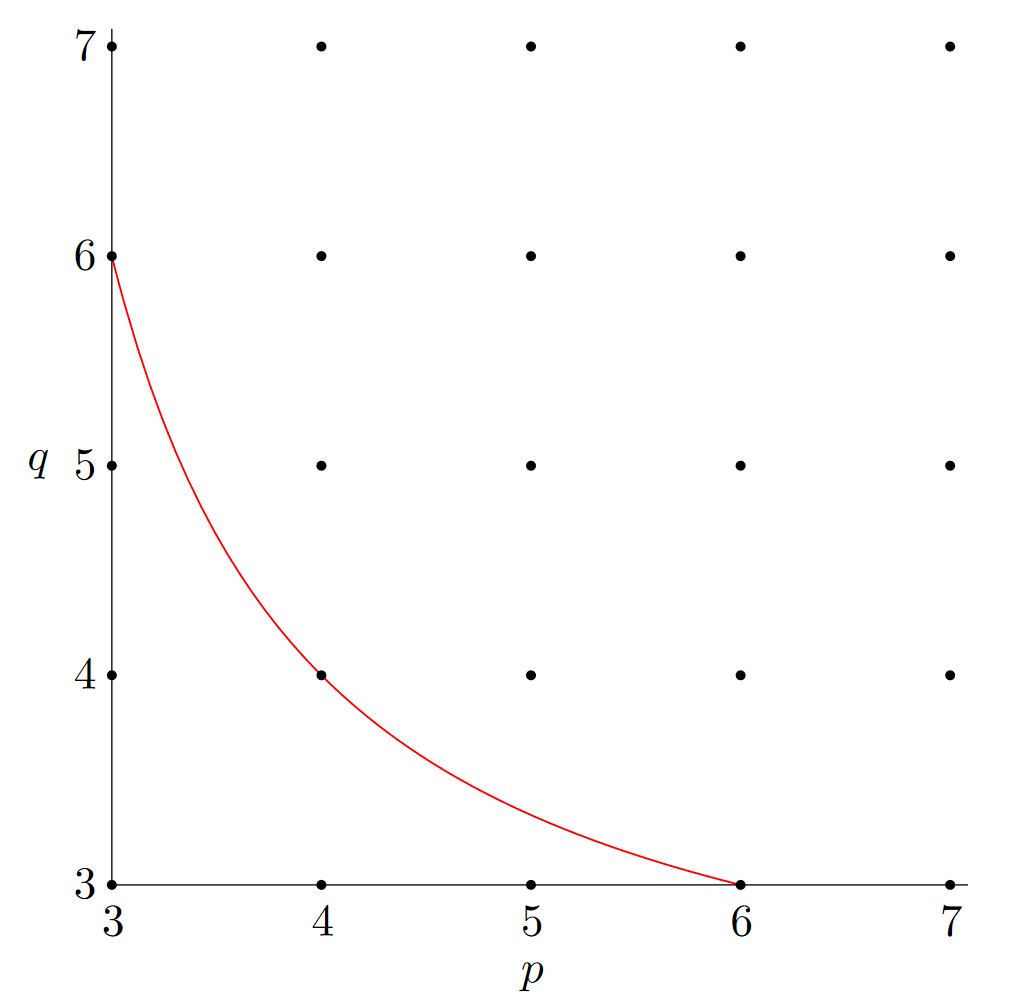
\includegraphics[width=0.5\textwidth]{Fig51}
\caption{A graph of the Euclidean tilings.} 
\end{figure}

\begin{multicols}{2}

This diagram is quite powerful in that it shows clearly the space of regular tilings in each geometry. Those on the line are Euclidean such as \(\{3,6\}\), those below the line are elliptic such as \(\{3,4\}\), and the infinity of those above it are \textit{all} hyperbolic! With so many, one would hope that there would be a way of visualising or creating images of these tilings---thanks to the work of Henri Poincar\'{e} and Felix Klein, you can look at visualisations of the hyperbolic plane.

Both of them act as a projection of the hyperbolic plane to the unit disk\footnote{The set of points on the Euclidean plane of distance less than or equal to 1 from \((0,0)\).} where the edge of the disk can be seen as the "edge at infinity" of the hyperbolic plane---although I will not mention the specifics of geometric constructions or calculations with them in this article, it should be clear that distances in the disk going out from the centre become increasingly large for the corresponding hyperbolic figures. In the Poincar\'{e} disk model, lines are represented by circle arcs drawn in the disk which are orthogonal to the disk's edge and the model represents angles accurately (this property of a mapping from one space to another is known as \textit{conformality}). In the Klein model, conformality is lost with the benefit that lines are drawn straight here. The same \(\{7,3\}\) tiling is represented using the two models in \textbf{Fig. 3.6}---though in general the images I will use in this article and any articles involving hyperbolic space in the future will use the Poincar\'{e} disk model due to its angle preserving nature.

Another incredible object that can exist in hyperbolic tilings is the \textit{apeirogon} or \(\infty\)-gon (a polygon with an infinite number of sides). In Euclidean tilings the only way it can be represented is in "degenerate"\footnote{The word \textit{degenerate} is used in mathematics to describe objects or situations which technically fulfill specific requirements but are so devoid of structure or meaning that they are worthless to study. Another example of a degenerate object would be the 2-sided or 1-sided polygons (which, on the Euclidean plane, are just straight lines).} tilings, such as can be found in \textbf{Fig. 3.7}, where the "sides" of the polygon are just an infinitely long line separated by dots denoting vertices at regular intervals. The image can be seen as a tiling of the Euclidean plane by 2 apeirogons.

However, hyperbolic space is sufficiently curved and "large" that apeirogons can exist as discrete shapes surrounded by other polygons and that, equally, there can be tilings with an infinite number of polygons around each vertex, such as those shown in \textbf{Fig. 3.8}! In this case, all the vertices of the tiling are actually points at the edge of the disk and thus at infinity, known as \textit{ideal points}.

\end{multicols}

\begin{figure}[h]
\centering
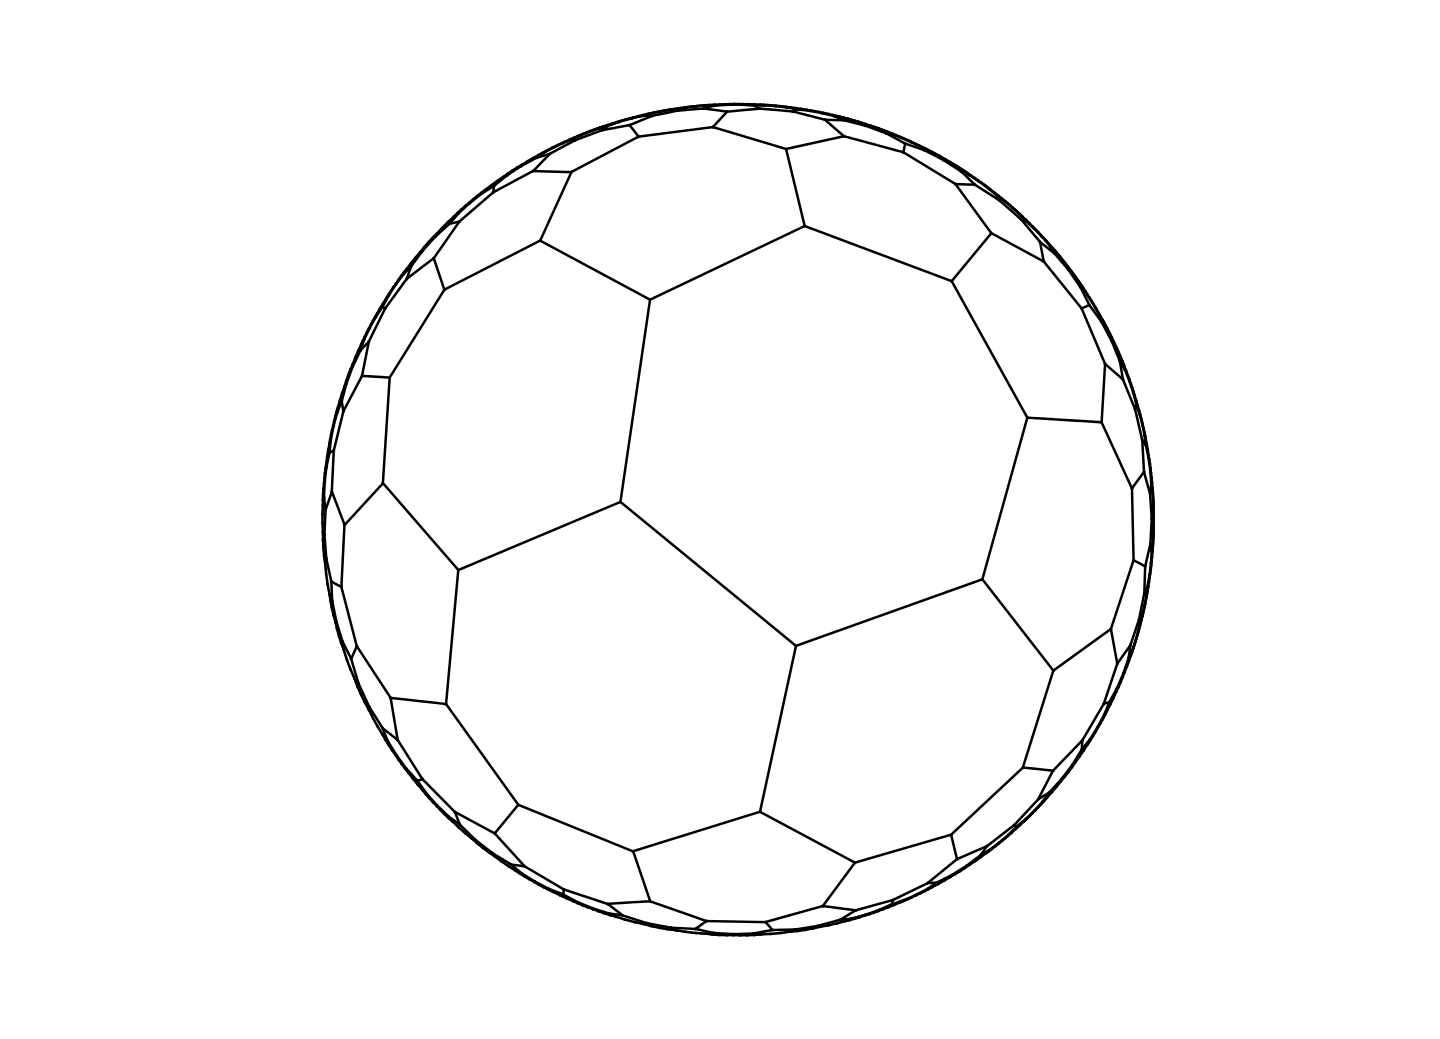
\includegraphics[width=0.3\textwidth]{Fig61}
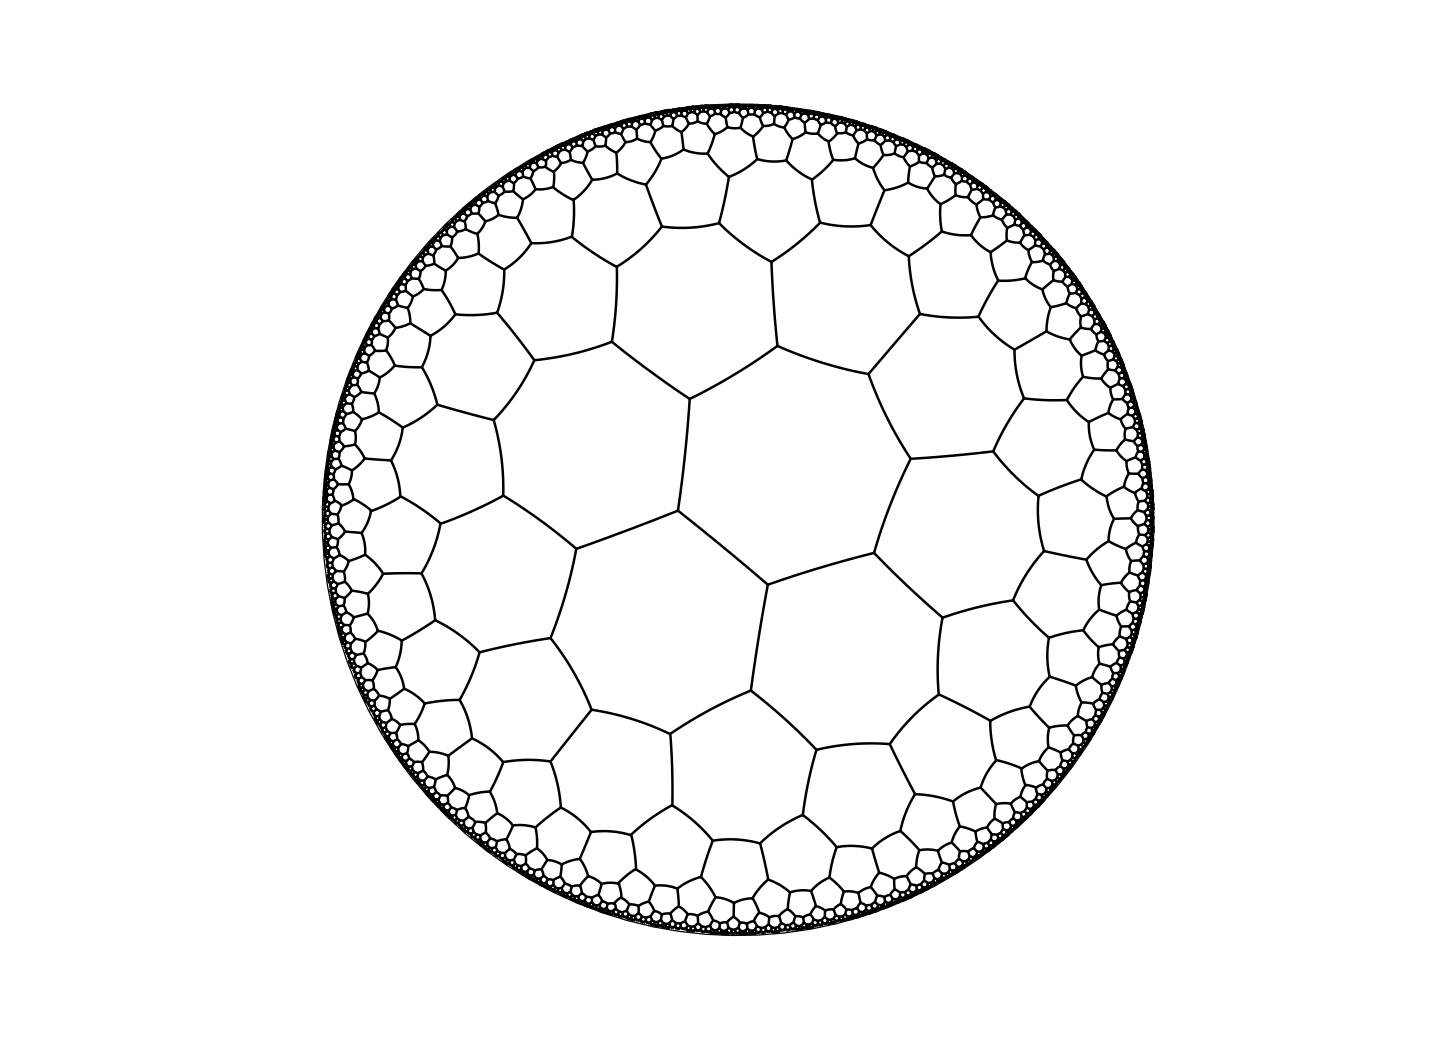
\includegraphics[width=0.3\textwidth]{Fig62}
\caption{A \(\{7,3\}\) tiling projected into the Klein Model and the Poincare Model.} 
\end{figure}

\begin{figure}[h]
\centering
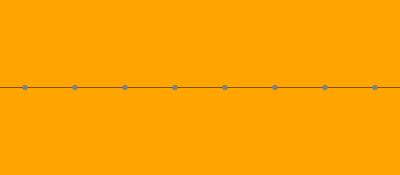
\includegraphics[width=0.5\textwidth]{Fig71}
\caption{A \(\{\infty,2\}\) tiling.} 
\end{figure}

\begin{figure}[h]
\centering
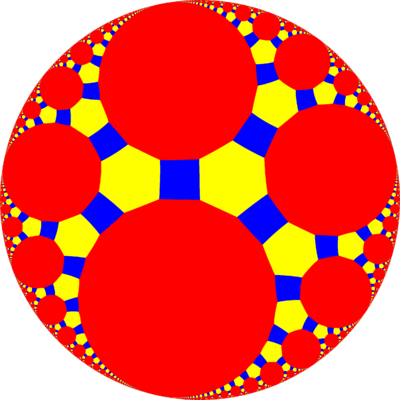
\includegraphics[width=0.25\textwidth]{Fig81}
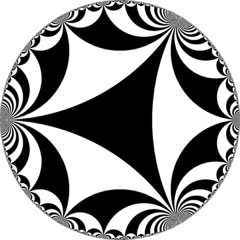
\includegraphics[width=0.25\textwidth]{Fig82}
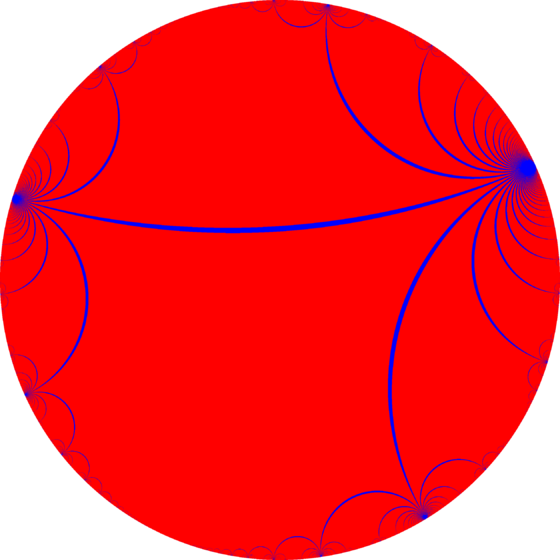
\includegraphics[width=0.25\textwidth]{Fig83}
\caption{A tiling of apeirogons with squares and hexagons, the \(\{3,\infty\}\) tiling and the \(\{\infty,\infty\}\) tiling.} 
\end{figure}

\section{Higher-dimensional Hyperbolic Space, Horocycles and beyond...}

\begin{multicols}{2}

Hyperbolic geometry becomes even more complicated in 3-space, or 4 or further! In order to investigate these spaces we need to understand the extended definition of the Schl\"{a}fli symbol and learn about \textit{horocycles}. In general, the Schl\"{a}fli symbol \(\{x_n, x_{n-1},...,x_2,x_1\}\) denotes \(x_1\) copies of \(\{x_n, x_{n-1},...,x_2\}\) around each vertex---this allows us to talk about regular \textit{honeycombs} of arbitrary dimensions! You can see some examples of different cube-based polyhedron packings in \textbf{Fig. 3.9}, going from the elliptic to the hyperbolic (represented here by the Poincar\'{e} \textit{sphere} model).

Most interesting, however, is the next in the series, namely \(\{4,3,6\}\), whose vertices are purely ideal. To see why \(\{4,3,6\}\) would suddenly have only ideal vertices while all its predecessors have none, we can look at its \textit{dual honeycomb}. The dual of a honeycomb is formed by taking the geometric centres of every face of every polyhedron involved and drawing lines between those that are adjacent to each other (as in, those which are part of a common polyhedron). 2D examples are easier to visualise at first, so let's take a look at some: in \textbf{Fig. 3.10}, we see two diagrams, one showing how the square tiling \(\{4,4\}\) is self-dual, where the original tiling is in blue and the dual is in red, the second showing how the dual of the cube (corresponding to the Schl\"{a}fli symbol \(\{4,3\}\)) is the octahedron (with symbol \(\{3,4\}\). Can you spot a pattern here?

The dual of a geometric structure defined by the symbol \(\{x_n, x_{n-1},...,x_2,x_1\}\) is \(\{x_1, x_2,...,x_{n-1},x_n\}\)! Can you think why this is? 

It allows us to see that the dual of \(\{4,3,6\}\) is \(\{6,3,4\}\), which can be interpreted as having 4 of the polyhedron \(\{6,3\}\) around a point... except that \(\{6,3\}\) defines the normal Euclidean hexagonal tiling of hexagons... Remarkably, hyperbolic space is so curved that it permits Euclidean tilings as infinite-sided polyhedra where the plane curves in on itself and becomes a form of hyperbolic ball---such an object is known as a \textit{horocycle}\footnote{The official definition of a horocycle is a curve in hyperbolic space with the property that all lines intersecting it orthogonally tend to the same ideal point, but for our purposes the above commentary will suffice.} and to me it's simply astounding that such an object could exist. Consequently, since the definition of a dual honeycomb \(B\) of a honeycomb \(A\) requires that the number of faces of the polyhedra in \(B\) is the same as the number of the edges going into the vertices of \(A\), it follows that there are infinite number of lines going into the vertices of \(\{4,3,6\}\) and thus its vertices are ideal.

\end{multicols}

\begin{figure}[h]
	\centering
	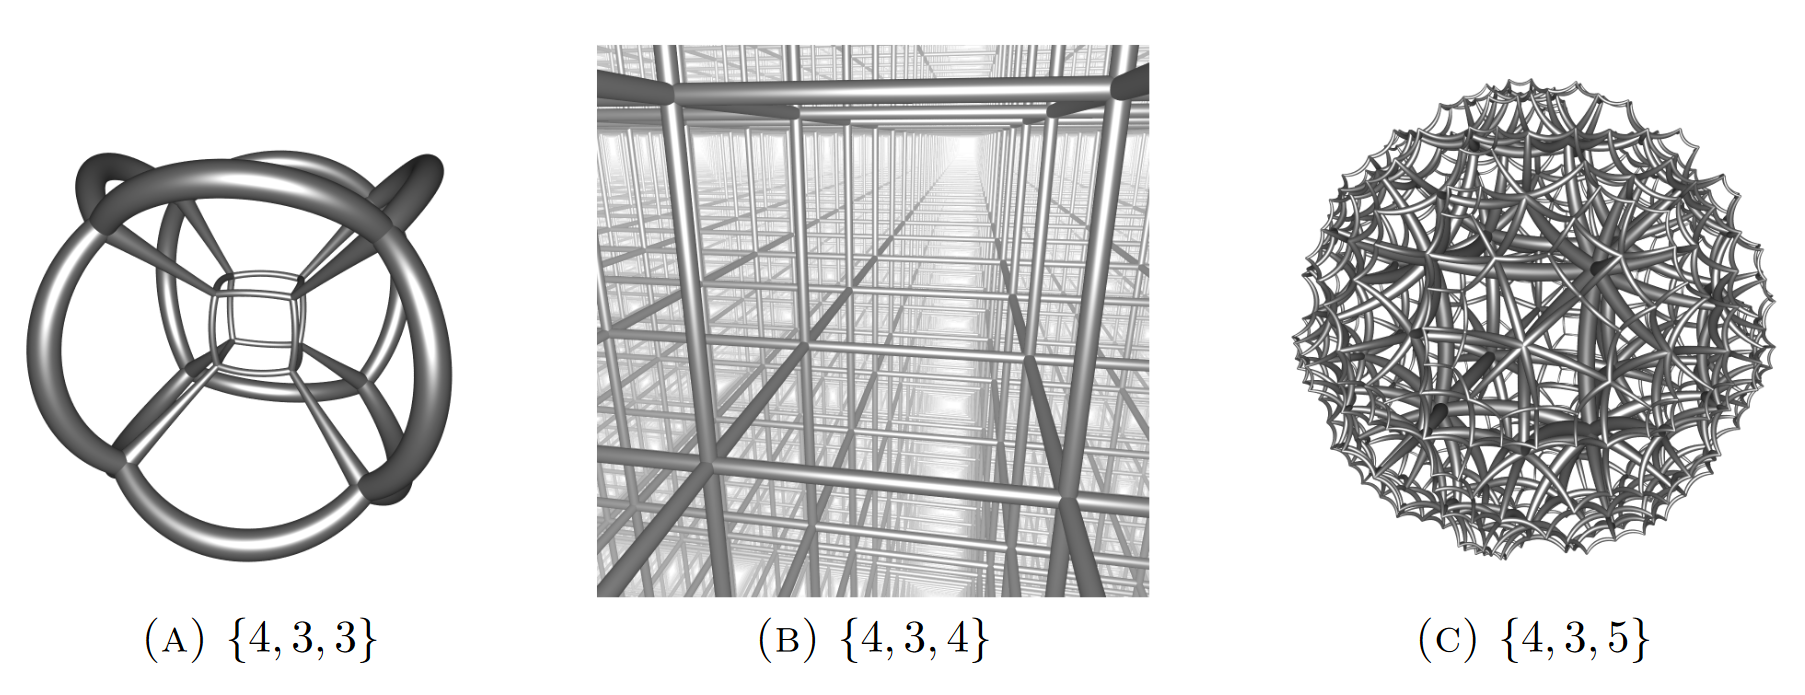
\includegraphics[width=0.5\textwidth]{Fig91}
	\caption{A series of three poyhedron packings in different spaces with their respective Schl\"{a}fli symbols.} 
\end{figure}

\begin{figure}[h]
	\centering
	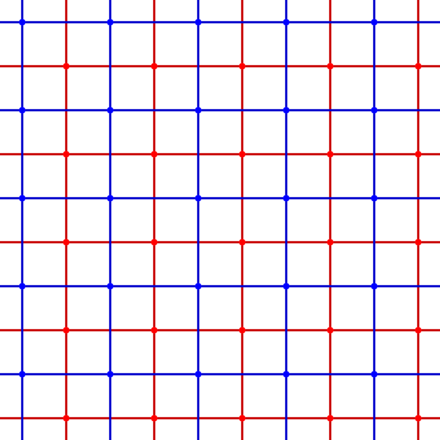
\includegraphics[width=0.4\textwidth]{Fig101}
	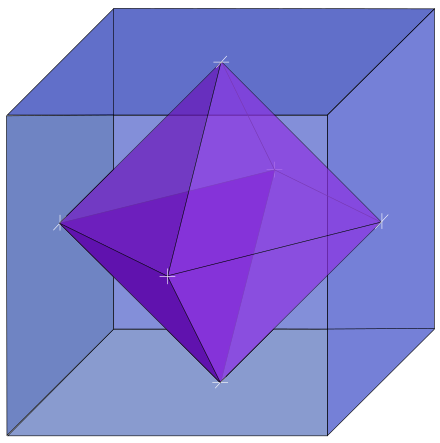
\includegraphics[width=0.4\textwidth]{Fig102}
	\caption{The duals of \(\{4,4\}\) and \(\{4,3\}\).} 
\end{figure}

\begin{multicols}{2}

Modern-day geometry is even stranger than much of what we have talked about here. Instead of studying simply the Euclidean plane, one studies general \textit{affine planes}, for which Euclid's first and fifth axiom hold along with the requirement:

\begin{itemize}
\item There are four points such that no line is incident with more than two of them.
\end{itemize}

and instead of studying the elliptic plane, mathematicians examine \textit{projective planes}, in which Euclid's first axiom holds, there are no parallel lines and the above requirement holds. Further, both of the planes just mentioned can be realised using any number system (or for those who know some abstract algebra, any \textit{field})---for example, one can create the affamed Complex Projective Plane by considering \(\mathbb{C}^3\) and then calling the set of lines going through the origin "points" or, equivalently, saying that two points \((x_1,x_2,x_3)\) and \((y_1,y_2,y_3)\), with \(x_n,y_n \in \mathbb{C}\), are "the same" if there is some complex number \(z\) so that \((zx_1,zx_2,zx_3) = (y_1,y_2,y_3)\). In this odd world where points' coordinates are described using complex numbers and lines are planes intersecting the origin, one can have many objects that we could never have in our own geometries such as the 3-dimensional surfaces known as \textit{3-folds}---these exist in Complex Projective 4-space and often have so many rotational or complex symmetries that they simply have no analogue in our universe.

For those of you that have enjoyed this article, you may wish to read up on \textit{differential geometry}, in which \textit{Riemannian manifolds}, a generalisation of traditional geometric surfaces to any number of dimensions and which only have the requirement that areas "near" each point act analogously to Euclidean space\footnote{The official definition is a \textit{topological space} which has a neighbourhood associated with every point that is \textit{homeomorphic} to some Euclidean \(n\)-space equipped with a useful object for measuring distances known as a \textit{Riemannian metric}, but that's for extra reading!}---it has really allowed mathematicians to better grasp what "spaces" \textit{are} and the various properties that they could have... Riemann himself was the top student of Gauss and formulated the above concepts after being introduced to Gaussian curvature by his mentor! So, for further reading, look up:

\begin{itemize}
\item The notion of a \textit{field} in abstract algebra and how they are used in the definitions of \textit{projective} and \textit{affine planes}.
\item \textit{Topological} spaces.
\item \textit{Uniform tilings} of the hyperbolic plane; there's an excellent Wikipedia page on this that contains many more images than in this article!
\item \textit{Riemannian} geometry; although you shouldn't expect to pick this up immediately, since it is a complex subject, true understanding of this should make General Relativity easy to read!
\item Hypercycles and the actual definition of horocycles
\item \textbf{Definitely}, if nothing else, go to "h3.hypernom.com" and try and use your arrow keys and WASD to move around---it's a simulator of hyperbolic 3-space from within the Poincar\'{e} sphere.
\end{itemize}

\end{multicols}

\section{Challenge V}

\begin{multicols}{2}

And now, as per usual the challenge with a relatively simple first part and a second part that I know \textit{no} good solutions to---if you have solutions to either of these, please email either \textbf{Isky Mathews} or \textbf{Benedict Randall Shaw} with them!

\begin{itemize}
\item What structure does the symbol \(\{5,3,4\}\) describe?
\item Can you come up with a notation for tilings, polyhedra and honeycombs which works for \textit{non-regular}, \textit{non-vertex transitive} structures?
\end{itemize}

\end{multicols}